\section{a}

\subsection{1 + 3}

This values were compared with the example seen in class.

\begin{itemize}
    \item ANDC too high -> high coupling, adding features more difficult, maintenance, subclass coupling
    \item AHH too high -> takes more time to compute (overloading) + \^ TO MUCH INHERITANCE
    \item NOM/NOC -> see below + small project -> not many methods -> ++ maintenance extensible
    \item LOC/NOM -> few methods per class but many lines per method => shoud refactor to have more modular methods -- maintenance extensible
    \item CYCLO/LOC -> flat code -> good because less tests -> mainly adding/storing data -> declarative language ??? ++ maintenance extensible
    \item CALL/NOM -> high but low FANOUT/CALL denotes that mostly operations from same class are called. so good coupling ++ maintenance extensible
    \item FANOUT/CALL -> low coupling thanks to facades ++ maintenance extensible
\end{itemize}

scores well on CYCLO NOM FANOUT

\subsection{2}
\begin{itemize}
    \item ANDC : average number of derived classes
    \item AHH : average hierarchy height
    \item NOM/NOC : number of methods / class
    \item LOC/NOM : number of lines of code / method
    \item CYCLO/LOC : proportion of lines of codes that are conditional branchement
    \item FANOUT : number of classes called in operations
    \item CALL : number of operations called from other operations (only one is counted per operation)
\end{itemize}

\subsection{4}

\begin{figure}[h]
    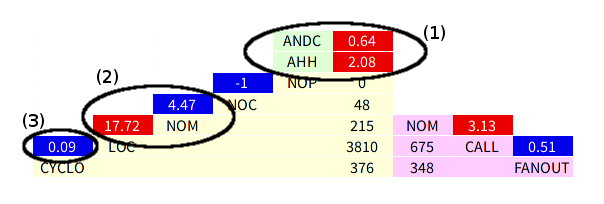
\includegraphics{OverviewPyramid_annotated.png}[width=\textwidth]
    \caption{\label{fig:pyramid}Overview pyramid with emphasis on important points}
\end{figure}

\begin{enumerate}
    \item Hierarchy is too big in both width and height. It denotes a strong coupling. The same features could probably be reached without inheritance
    \item Number of methods is good because it is not high but number of lines of code is too high. This could be fixed by splitting methods into smaller ones.
    \item Not many conditional branchements is very good for testing (both unit tests and integration tests) and to read and understand the code.
\end{enumerate}

\section{b}

\section{c}